\section{Introductie}

\ifx\aanleiding\undefined
\newcommand{\aanleiding}{}

\begin{wrapfigure}{r}{4cm}
  \begin{center}
    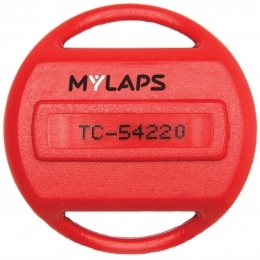
\includegraphics[width=4cm]{style/images/transponder}
  \end{center}
  \caption{MyLaps ProFlex transponder, op schaal}
  \label{fig:transponder}
  \vspace{15mm}
\end{wrapfigure}

In baansporten is de laatste jaren een ontwikkeling gaande om tijdregistratie te digitaliseren door het gebruik van transponders (bijvoorbeeld de MyLaps ProFlex transponder in Figuur~\ref{fig:transponder}) en detectie-lussen (Figuur~\ref{fig:detection-loop}) in de baan. Door deze ontwikkeling zijn nieuwe mogelijkheden ontstaan om ook naast het wedstrijdmoment de sportprestaties in te zien. Het constateren van de hierna genoemde nieuwe mogelijkheden was de aanleiding van dit project.

\begin{wrapfigure}{r}{4cm}
  \begin{center}
    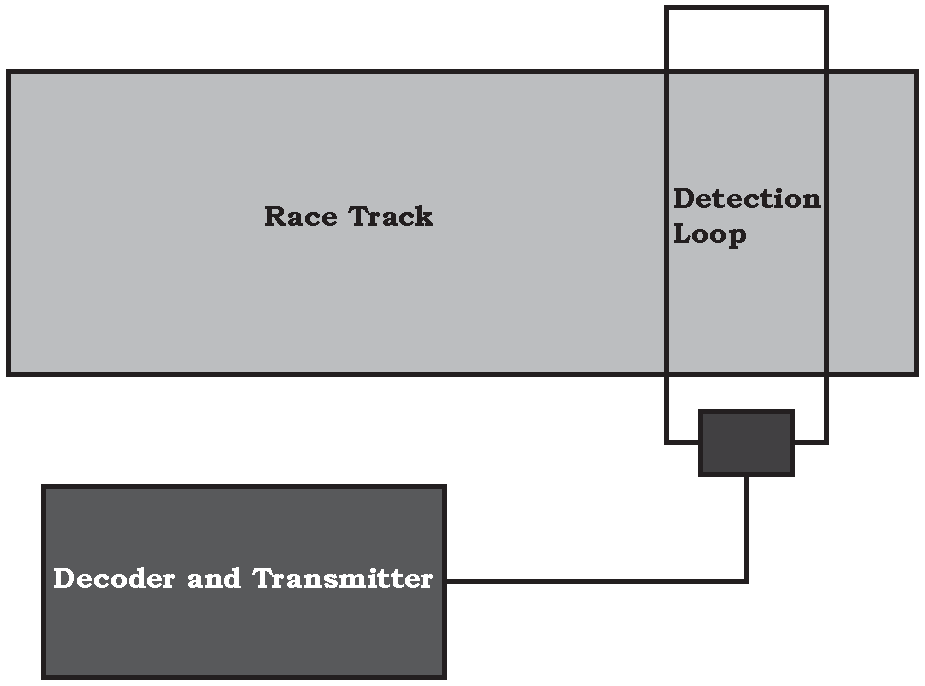
\includegraphics[width=4cm]{style/images/DetectionLoop}
  \end{center}
  \caption{Een schema van een detectielus en en decoder}
  \label{fig:detection-loop}
  \vspace{5mm}
\end{wrapfigure}

Een grote speler op de tijdregistratie-markt is MyLaps\footnote{\url{http://www.mylaps.com}}. Dit bedrijf installeert en beheert detectie-lussen en is actief bij diverse sporten zoals schaatsen, wielrennen, zwemmen, atletiek en diverse motorsporten. Bij sporten met permanente banen liggen de detectie-lussen het gehele jaar in de baan. Er bestaat de mogelijkheid om op de website van MyLaps doorkomst-tijden in te zien. De informatie die uit deze tijden is af te leiden, wordt door sporters als erg waardevol gezien om zich willen blijven verbeteren, waardoor er steeds meer getraind wordt met deze transponders.

\begin{figure}
  \begin{center}
    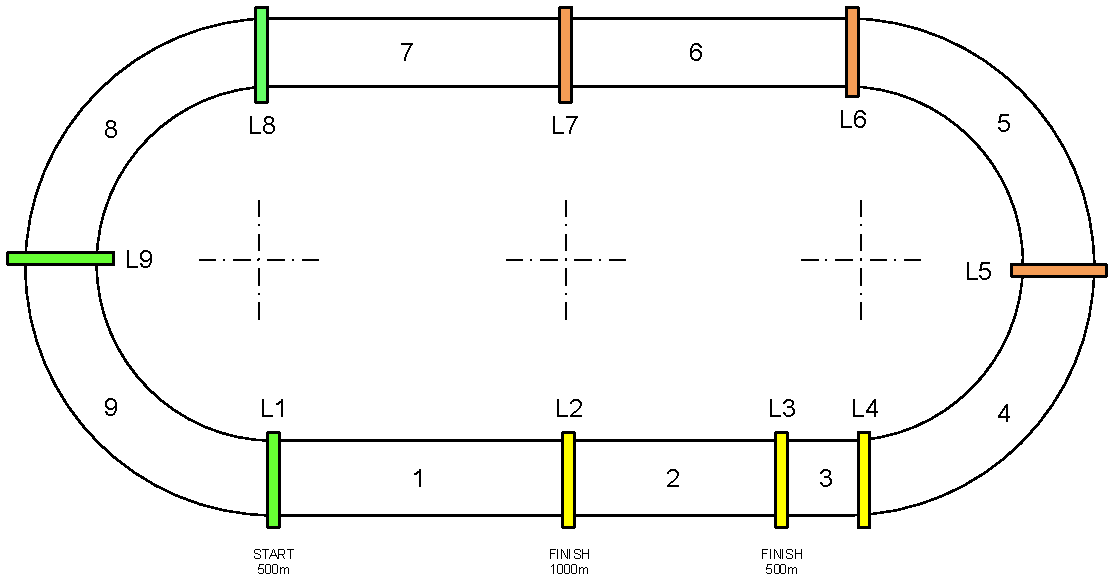
\includegraphics[width=0.8\textwidth]{style/images/BaanoverzichtHaarlem}
  \end{center}
  \caption{L1 tot en met L9 zijn de negen MyLaps transponderlussen in Haarlem}
  \label{fig:track-transponders}
\end{figure}

Voor aanvang van het seizoen worden door MyLaps detectielussen geïnstalleerd. De lussen bevinden zich in het ijs of onder het houten oppervlak van een baanwielrenbaan. Elke lus heeft een elektromagnetisch veld. Wanneer een sporter met transponder over dat veld heen rijdt, wordt de transponder geactiveerd en stuurt deze een unieke puls, die de lus opvangt. De MyLaps X2 server die aan de lussen zit aangesloten stuurt vervolgens het signaal door naar de MyLaps Cloud.

Het huidige gebruik van transponders - buiten wedstrijden - is voornamelijk achteraf, terwijl juist tijdens de training zowel sporter als coach het meeste bezig zijn met de prestaties. Het is daarom wenselijk om de resultaten in real-time door te geven aan coaches en sporters zelf.

Op veel banen zijn meerdere detectie-lussen geïnstalleerd, terwijl er op de website van MyLaps slechts één wordt ontsloten. In Thialf, de schaatsbaan in Heerenveen, Friesland, liggen bijvoorbeeld twaalf detectie-lussen, in Haarlem (Figuur~\ref{fig:track-transponders}) negen en op de andere schaatsbanen liggen er tenminste twee. Door de data van meerdere lussen te combineren is een betere indicatie te maken van de snelheid van sporters.

\begin{wrapfigure}{r}{0.4\textwidth}
 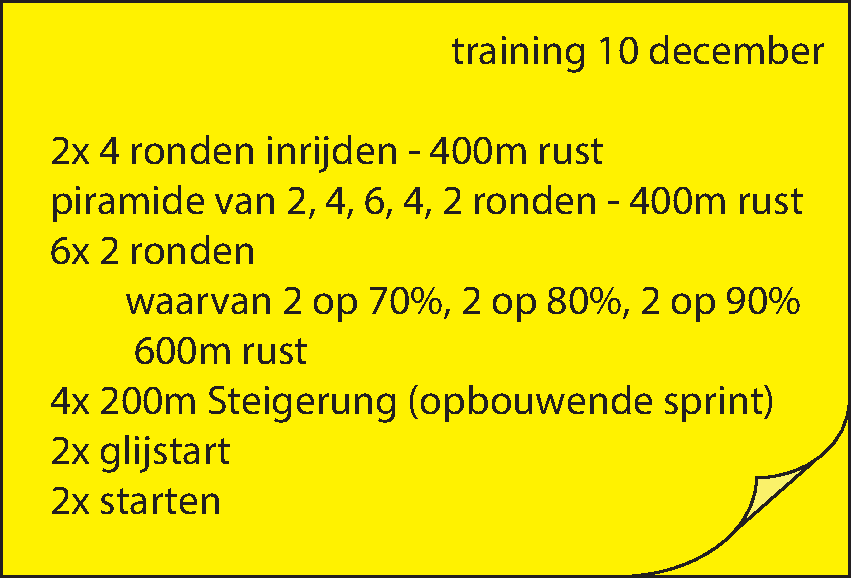
\includegraphics[width=0.4\textwidth]{style/images/training}
 \caption{Een typisch schaats-trainingsschema}
\end{wrapfigure}

Trainingen, bij bijvoorbeeld schaatsen, bestaan uit losse trainingsonderdelen. Allround schaatsers moeten bijvoorbeeld 4 ronden warmrijden, dan 6 keer 2 ronden sprinten, dan 4 keer een sprintje van 200 meter, 2 keer een glijstart en dan 2 keer een echte start bij de coach, vanuit de zijkant van de baan. Tussendoor is er rust, zo is het gebruikelijk om na een opdracht tenminste 400 meter uit te glijden. Het verschil tussen training en rust is af te leiden uit de verhouding tot de maximale snelheid.

Veel trainingselementen bestaan dus uit korte opdrachten, waar het juist om snelheid gaat. Een enkele lus is dan niet afdoende, omdat de rust voor of na de opdracht mee wordt gewogen. Sporters starten en stoppen namelijk niet precies boven de lus, maar starten vaak na de bocht en stoppen afhankelijk van de afstand van de opdracht op een willekeurig punt. 

Andere trainingen van bijvoorbeeld lange afstands- of marathonschaatsers kunnen bestaan uit één element: de hele training lang schaatsen, zonder overeind te komen. Wanneer er op tactische punten detectie-lussen geïnstalleerd zijn, is er bijvoorbeeld ook onderscheid te maken tussen bochten en de rechte stukken. Bij sporten met een ronde baan verschilt de snelheid in de bocht namelijk erg met die op het rechte eind. Deze vergelijking gebeurt nu al in Thialf, in het professionele circuit tijdens wedstrijden op televisie.

Topsporters zijn enorm prestatiegericht en als je al aan de top zit, dan kunnen kleine aanpassingen aan je techniek, ademhaling et cetera, grote verschillen maken. Coaches van professionele teams houden zich daarom bezig met allerhande analyses. Naast ademanalyse en hartslag monitoring, is het in Thialf bijvoorbeeld ook mogelijk om (van maximaal 20 schaatsers) continu de positie te bepalen met een in-door positioning system (IPS) ontwikkeld door InnoSportLab\footnote{\url{http://www.innosportlabthialf.nl}}.

Al deze geavanceerde analyses zijn echter te duur en kosten te veel tijd voor recreatieve sporters. MyLaps X2 biedt in combinatie met ons eindproduct recreatieve sporters toch een manier om analyses uit te voeren en zich naar een hoger niveau te tillen.
\fi

Aan de hand van de projectopdracht, ons Plan van Aanpak (te vinden in Appendix~\ref{ch:plan-van-aanpak}) en gesprekken met Johan en Cor-Paul hebben we dit Ori\"entatieverslag opgesteld. Dit verslag biedt inzicht in de mogelijke technieken voor het ontwikkelen van mobiele applicaties en server back-ends, geschikt voor onze toepassing. Ook zullen in dit verslag de keuzes voor het gebruik van bepaalde technieken worden toegelicht.

\section{Soortgelijke oplossingen}

\ifx\vergelijkbaresystemen\undefined
\newcommand{\vergelijkbaresystemen}{}
\label{sec:vergelijkbare-systemen}

Er bestaan al enkele oplossingen die functionaliteit bieden die vergelijkbaar is met die van de applicatie die wij gaan bouwen. Strava (figuur~\ref{fig:strava}) en RunKeeper (figuur~\ref{fig:runkeeper}) maken gebruik van GPS om onder andere hardlopers en wielrenners van realtime informatie te voorzien. \mylaps Practice (figuur~\ref{fig:mylapspractice}) is een website waar je na je training je prestaties kan terugkijken. Er bestaat ook een iPhone App voor \mylaps Practice (figuur~\ref{fig:mylapspractice-app}). Coach Watch (figuur~\ref{fig:coachwatch}) is een iPad applicatie waarmee coaches hun teams kunnen volgen.

\begin{figure}[ht]
\centering
\subfigure[Strava]{
    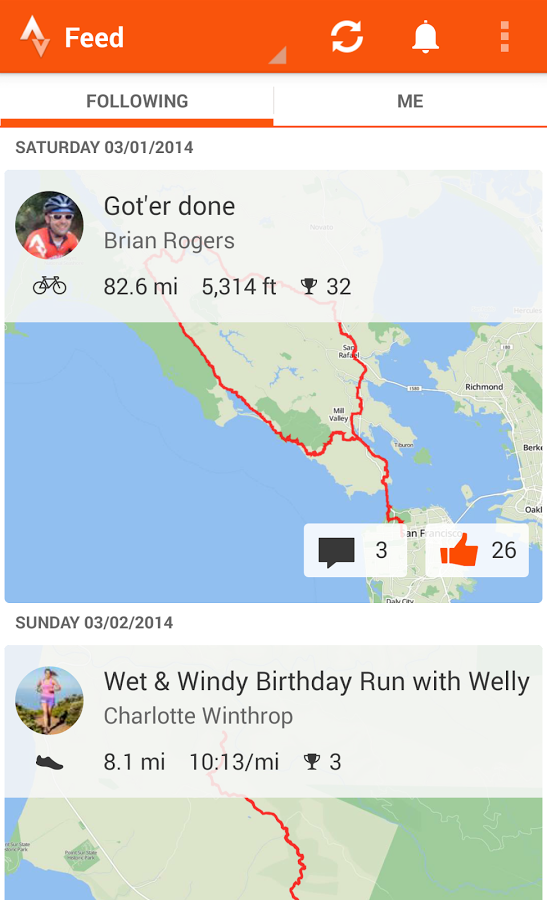
\includegraphics[height=5cm]{style/images/Strava}
    \label{fig:strava}
}
\subfigure[RunKeeper]{
    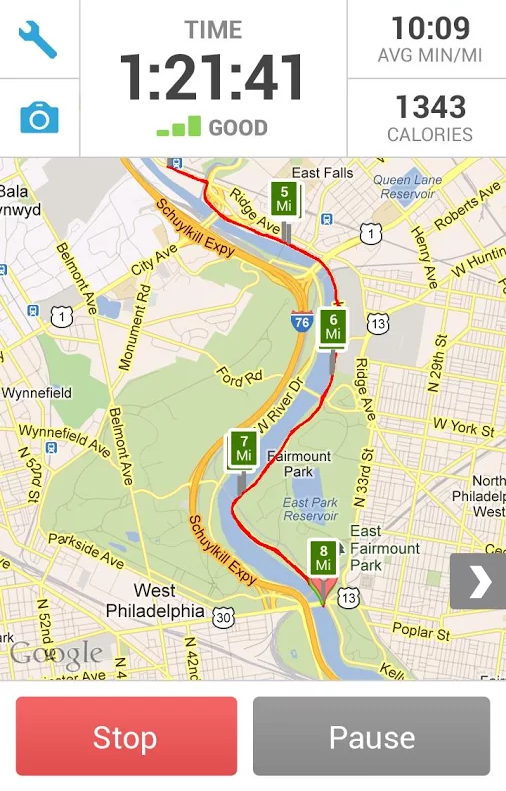
\includegraphics[height=5cm]{style/images/RunKeeper}
    \label{fig:runkeeper}
}
\subfigure[Coach Watch]{
    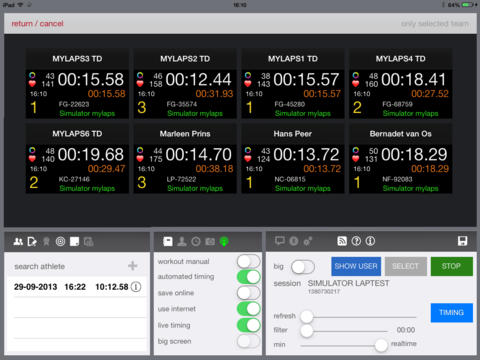
\includegraphics[height=5cm]{style/images/CoachWatch}
    \label{fig:coachwatch}
}

\subfigure[\mylaps Practice]{
    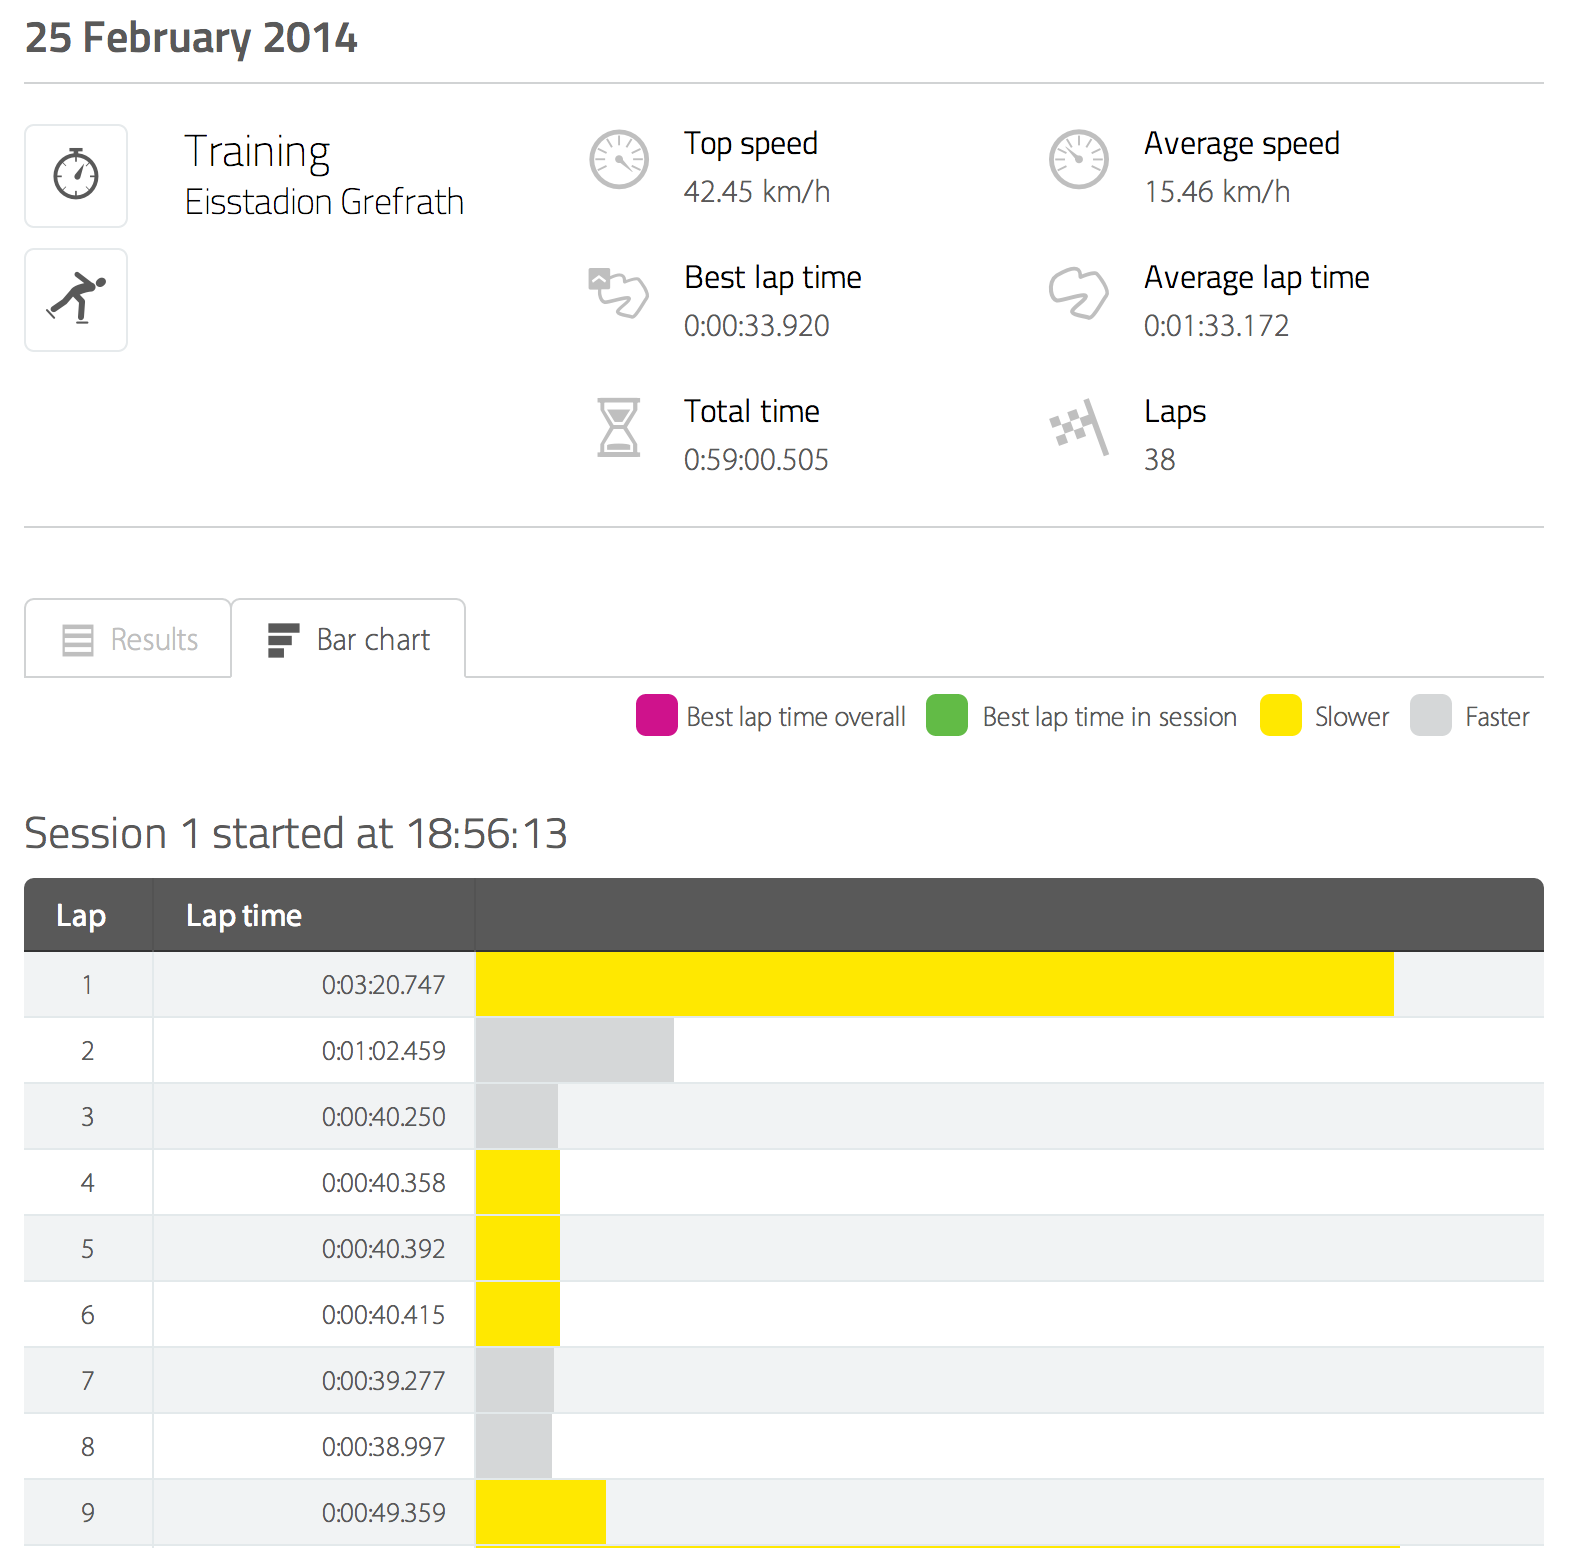
\includegraphics[height=7cm]{style/images/MyLapsPractice}
    \label{fig:mylapspractice}
}
\subfigure[\mylaps Practice App]{
    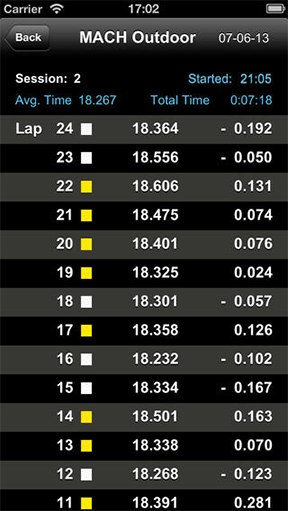
\includegraphics[height=7cm]{style/images/MyLapsPractice-App}
    \label{fig:mylapspractice-app}
}

\caption{Soortgelijke oplossingen}
\label{fig:soortgelijke-oplossingen}
\end{figure}

Strava en RunKeeper zijn voor baansporten, zoals bijvoorbeeld schaatsen, niet goed bruikbaar, aangezien GPS op de banen slecht presteert, waardoor de informatie niet nauwkeurig genoeg is. \mylaps Practice en Coach Watch maken wel gebruik van de detectielussen in de banen. De \mylaps Practice website kan alleen gebruikt worden voor het achteraf bekijken van sportprestaties en deze de applicatie is vooral gericht op motorsporten. CoachWatch is een (vrij dure) applicatie die vooral gericht is op coaches en dus minder geschikt voor trainingen of voor amateurschaatsers.

Emando ziet de mogelijkheid om een applicatie te bieden die gebruikmaakt van de detectielussen in de banen, die live gegevens kan tonen op een smartphone en die ook nog eens goedkoop of gratis is. Onze applicatie richt zich dus op het invullen van de stukken die missen in de bestaande oplossingen.
\else
In Sectie~\ref{sec:vergelijkbare-systemen} is een overzicht gegeven van soortgelijke oplossingen.
\fi

\section{Doelgroep \& gebruikers}

\ifx\doelgroep\undefined
\newcommand{\doelgroep}{}
\label{sec:doelgroep}

\subsection{Schaatsers}
De voornaamste doelgroep van onze applicatie zijn de recreatieve en amateur schaatsers. Zij moeten met behulp van onze applicatie meer inzicht krijgen in hun prestaties en trainingen. 
Om er voor te zorgen dat deze groep gebruikers onze applicatie verkiest boven de reeds bestaande (minder uitgebreide) systemen, dienen zij snel en gemakkelijk met de applicatie aan de slag te kunnen gaan.
Bij een té ingewikkeld systeem zullen zij afhaken en de overstap naar onze applicatie wellicht niet willen maken.
Omdat zij de belangrijkste doelgroep zijn van de applicatie, is het belangrijk dat zij gemotiveerd worden om de applicatie te blijven gebruiken en hen tevens motiveren om ook anderen aan te sporen dit te doen.
Met behulp van sociale componenten zoals trainingsgroepen, het volgen van andere schaatsers en leaderboards kan onze applicatie hen hierin stimuleren.
\subsection{Coaches}
Als tweede doelgroep zijn er de coaches van de schaatsers. Dit zijn mensen die de schaatsers begeleiden bij hun trainingen en wedstrijden. Zij beschikken zelf niet altijd over een transponder, omdat niet iedere coach zelf schaatst.
Zij willen graag snel en gemakkelijk inzicht in de data van de schaatsers die zij coachen. Het moet voor hen dus gemakkelijk zijn om snel tussen schaatsers te kunnen switchen en deze prestaties zowel onderling als per training gemakkelijk te kunnen vergelijken.
\subsection{Overige gebruikers}
Tot slot is er de groep gebruikers die zelf geen deel uitmaakt van de schaatswereld. Zij zijn geen schaatsers of coaches en zijn met name geïnteresseerd in de mogelijkheden van de applicatie en het volgen van kennissen of bekende schaatsersn.
Ook zij moeten in staat zijn om de applicatie gebruiken, weliswaar in mindere mate.
\else
In Sectie~\ref{sec:doelgroep} is behandeld wat de doelgroep van de applicatie is en welke verschillende soorten gebruikers er verwacht worden.
\fi

\section{Back-end}\label{sec:orientatie-back-end}
Afhankelijk van welk back-end platform we kiezen, zijn er verschillende mogelijkheden voor de servers waarop de back-end kan draaien. Ook is er de keuze tussen traditionele server clusters en een cloud-oplossing, zoals een \ac{paas}. Er zijn verschillende redenen om wel of niet voor een cloud oplossing te gaan. De voor- en nadelen van een cloud oplossing staan hieronder opgesomd.

Bij het vergelijken van een cloud oplossing met een traditioneel serverpark zijn we er vanuit gegaan dat dit serverpark zelf beheerd wordt en niet uitbesteed is wordt een externe partij. Dit houdt ook in dat het onderhoud hiervan door ons zelf gedaan zou worden.

\subsection{Schaalbaarheid}
Cloud oplossingen bieden de mogelijkheid om gemakkelijk en (automatisch) vrijwel onbeperkt te schalen bij een hoge load. Sommige cloud oplossingen zoals Windows Azure bieden de mogelijkheid om dit automatisch op te laten schalen aan de hand van de load. Bij een traditioneel serverpark is dit niet het geval. Hierbij dienen handmatig servers aangesloten te worden op het moment van een hoge load. 


\subsection{Besturingsssyteem}
In tegenstelling tot bij een traditioneel serverpark, ligt de verantwoordelijkheid van het beheren van de besturingssystemen niet bij ons, maar bij de beheerder van de cloud service. Het instellen en optimaliseren van alle besturingsssystemen voor alle frameworks en programmeertalen kan veel tijd kosten. Door deze verantwoordelijkheid bij de beheerder van de cloud service te  leggen, kan veel tijd bespaard worden.

\subsection{Onderhoud \& Uptime}
Cloud oplossingen worden beheerd en onderhouden door de service provider, waar dit bij een traditioneel serverpark bij ons zelf zou liggen. Ook bieden cloud oplossingen een gegarrandeerde hoge update, zonder dat we hier zelf iets voor hoeven doen.

\subsection{Kosten}
Bovenop de kosten van die de service provider van de cloud oplossing maakt, wordt een winstmarge geheven. Dit is bij het traditionele serverpark niet het geval. Bij een cloud oplossing zijn de onderhoudskosten (voor ons) vele malen lager, waardoor deze kosten zowel hoger als lager uit kunnen vallen in vergelijking tot de kosten van een traditioneel serverpark.

\subsection{Beschikbaarheid frameworks/programmeertalen}
Doordat cloud oplossingen door de service provider beheerd worden is er doorgaans minder vrijheid in het kiezen van frameworks/programmeertalen. Alleen de bekendste en meest gebruikte frameworks/programmeertalen worden ondersteund. Bij een traditioneel serverpark hebben we de mogelijkheid om deze volledig zelf in te richten en hebben we daarmee meer vrijheid. Vanwege onze keuze voor C\# en .NET, is dit geen probleem voor ons.

\begin{table}
\centering
\begin{tabular}{lccccc}
\textbf{}        & \multicolumn{1}{l}{\textbf{Azure}} & \multicolumn{1}{l}{\textbf{App Engine}} & \multicolumn{1}{l}{\textbf{AWS}} & \multicolumn{1}{l}{\textbf{Heroku}} & \multicolumn{1}{l}{\textbf{AppFog}} \\
\textbf{.NET}    & \times &        & \times &         &        \\
\textbf{Java}    & \times & \times & \times & \times  & \times \\
\textbf{Scala}   & \times & \times & \times & \times  & \times \\
\textbf{Python}  & \times & \times & \times &         & \times \\
\textbf{Node.JS} & \times &        & \times & \times  & \times \\
\textbf{PHP}     & \times & \times & \times &         & \times \\
\textbf{Ruby}    & \times &        & \times & \times  & \times \\
\textbf{Overig}  &        & Go     &        & Closure & Erlang
\end{tabular}
\caption {Vijf grote \ac{paas} providers en de talen en frameworks die ze ondersteunen} \label{tab:paas} 
\end{table}

Het nadeel dat de prijs hoger kan liggen kan worden afgezwakt en mogelijk worden omgebogen: om grote hoeveelheden gebruikers aan te kunnen moet een traditioneel server cluster groot zijn, terwijl een \ac{paas} automatisch kan schalen en dus op dal-momenten significant goedkoper kan zijn. We verwachten dat het gebruik van onze applicatie een piek zal vertonen in de avond en in het weekend, omdat er voornamelijk buiten werk en schooltijd gesport wordt. Er is voor onze applicatie dus meer dal- dan piek-belasting en we verwachten dus ook dat een \ac{paas} oplossing goedkoper zal zijn dan een cluster.

In tabel~\ref{tab:paas} ziet u een overzicht van de verschillende grote cloud platformen die er momenteel zijn, en de talen en frameworks die ze ondersteunen~\cite{paas-list-tomsitpro, azure-scala, aws}. Zoals in de tabel te zien is ondersteunen de meeste \ac{paas}\'s vele talen en frameworks. Microsoft Azure en Amazon AWS ondersteunen de 4 grote platformen .NET, Java, Python en NodeJS.

De bestaande systemen van Emando zijn gemaakt met het .NET framework en draaien voornamelijk in Microsoft Azure als Cloud Service. Aangezien MyLaps voor ons een belangrijke databron is en de MyLaps SDK alleen voor C\#/.NET beschikbaar is, kan er veel werk bespaard worden door ook deze programmeertaal en runtime te gebruiken. 

Bovendien heeft Emando een laag over de MyLaps SDK heen geschreven waardoor de SDK bruikbaar is met \acf{rx}. \ac{rx} - mede ontwikkeld door prof.dr. H.J.M. Meijer~\cite{meijer2011world} - is een manier om LINQ te gebruiken voor observeerbare collecties en asynchroon programmeren, twee eigenschappen waar we binnen de applicatie mee te maken gaan krijgen.

Bij onze keuze hebben ook de andere platformen overwogen, maar door de beperkte beschikbaarheid van de MyLaps SDK (alleen binnen .NET) en het gebruik van .NET door Emando waren dit minder bruikbare opties.

\subsection{Real-time}\label{sec:orientatie-real-time}
De trainingsapplicatie moet zonder dat de gebruiker de applicatie handmatig ververst de laatste doorkomsten binnenkrijgen en tonen. Ook moet de getoonde rondetijd up to date zijn, en niet een ronde tijd van een vorig rondje. De communicatie tussen de back-end en de clients moet dus real-time zijn. Real-time wil zeggen dat de server een update naar de client kan sturen. In `normaal' web verkeer kan de server niet op elk moment een bericht sturen naar de client. De server kan alleen reageren op een verzoek van de client, omdat de client geen vast IP-adres heeft en er standaard geen poort open staat. Pas wanneer de client een uitgaand verzoek heeft gaat er een poort open.

Een oplossing hiervoor is WebSockets: bij WebSockets blijft de verbinding open en dus de poort en kan de server op elk moment een bericht sturen, als er bijvoorbeeld een schaatser voorbij een detectie-lus komt. Een verbinding openhouden kost geheugen op de server en de server heeft dus een maximum aantal verbindingen dat hij kan openhouden. Er bestaan verschillende WebSocket frameworks die je het aanmaken en onderhouden van de verbindingen uit handen nemen. Een hiervan is SignalR voor .NET. Emando heeft SignalR\footnote{\url{http://www.asp.net/signalr}} succesvol gebruikt tijdens de Olympische Spelen van 2014 om \url{http://live.schaatsen.nl} te voorzien van live data. SignalR is inmiddels een officiele ASP.NET library en wordt ontwikkeld en ondersteund door Microsoft ontwikkelaars.

\section{Client}
Er zijn tegenwoordig diverse manieren om mobiele applicaties te maken, voor diverse platformen (iOS, Android, Windows Phone). Deze verschillende methodes vereisen verschillende programmeertalen en architecturen. Een groot verschil tussen de verschillende methodes is de hoeveelheid code die kan worden hergebruikt tussen verschillende platformen. De uitersten hiervan gebruiken een compleet gescheiden broncode ten opzichte van een volledig gedeelde broncode. De volgende methodes zijn meegenomen in onze ontwerpkeuze:

\begin{description}
\item[Native applicatie:] Een native applicatie is een applicatie die ontworpen is voor een specifiek platform. Het design van dergelijke applicaties ligt (meestal) in het verlengde van de richtlijnen voor dit platform en het gebruik van platform specifieke handelingen (gestures) wordt gestimuleerd en gehanteerd binnen de applicatie. Vanwege de richtlijnen en het gebruik van deze gestures, zijn dergelijke applicaties zelfverklarend voor eindgebruikers. Een ander voordeel is dat door de native implementatie, de user interface performance van dergelijke applicaties doorgaans erg goed is.

Een nadeel van native applicaties is dat applicatie code vaak in een platform specifieke programmeertaal wordt ontwikkeld en dat er daardoor 3 complete applicaties ontwikkeld moeten worden om de drie grootste platformen te ondersteunen (iOS, Android en Windows Phone). Het ontwikkelen hiervan kost daardoor vaak veel tijd.
    
\item[Web applicatie:]
Een web applicatie is een applicatie die ontworpen is om op alle (mobiele) platformen te draaien. Deze applicatie is benaderbaar via het web (m.b.v. browsers) en heeft als groot voordeel dat deze maar 1x ontwikkeld hoeft te worden. Ook zijn veel ontwikkelaars bekend met de programmeertalen waarmee gewerkt moet worden (HTML, CSS en JavaScript).
    
Er zijn veel verschillende frameworks om mobiele applicaties te maken en daar ligt ook meteen een groot gevaar: elk framework heeft zijn eigen voordelen en wisselen tussen frameworks kan vaak betekenen dat grote delen van de applicatie opnieuw geschreven moeten worden. Ook tijdens ons project zijn diverse frameworks (Meteor, Angular, Backbone, Ember) ter sprake gekomen en voor elk genoemd framework wist er een projectlid voor- en nadelen te noemen.
    
\textbf{Frameworks:} jQuery Mobile~\cite{jq-mobile}, Sencha Touch~\cite{sencha}, Meteor~\cite{meteor}, AngularJS~\cite{angular}, Backbone.js~\cite{backbone}, Ember.js~\cite{ember}, Ionic~\cite{ionic}, React~\cite{React}
    
\item[Native applicatie met WebView:] Een ander belangrijk nadeel van web applicaties is het feit dat deze niet vindbaar zijn in de app stores. Native applicaties met een WebView\footnote{Een WebView is een soort van browser binnen een applicatie, zonder de mogelijkheid zelf een url in te voeren.} zijn applicaties waarin met behulp van een webview een reeds bestaande web applicatie geladen wordt. Hiermee kan met relatief weinig tijd worden meegeleund op het model van de applicatie winkels en is de applicatie in een klap vindbaar op de plek waar gebruikers zoeken naar applicaties.
    
Een nadeel van deze applicaties is hun performance. De applicatie laadt steeds webpagina's in en bij het wegvallen van de verbinding kan de applicatie doorgaans geen of weinig informatie of user interface tonen. Ook kan er doorgaans geen of weinig gebruik gemaakt worden van gestures. In sommige implementaties van deze applicaties wordt een onderscheid gemaakt tussen de offline user interface en de online web app, wat de performance verbetert en het probleem met het wegvallen van de verbinding oplost. De prestaties, vormgeving en gestures zijn echter vele malen minder praktisch ingericht dan bij een native applicatie. Het uitbrengen van een applicatie binnen de applicatie winkels brengt echter wel verwachtingen met zich mee. Doorgaans gaan gebruikers er vanuit dat de bovenstaande beschreven eigenschappen wel verwerkt zitten binnen deze applicaties.   
\textbf{Frameworks:} PhoneGap/Cordova~\cite{cordova}, Titanium~\cite{titanium}
    
\item[Cross Compiling: ] Cross Compiling is een techniek om broncode om te zetten naar uitvoerbare bestanden voor de verschillende platformen. Hiermee kan vaak de business- en servicelaag van de applicatie gedeeld worden tussen platformen, en sommige `cross-compilers' ondersteunen ook het delen van de presentatielaag. Vaak is dit echter niet wenselijk, omdat juist op de presentatielaag veel verschil gemaakt kan worden tussen platformen, om beter aan te sluiten bij de verwachtingen van de gebruiker. Met cross compiling wordt tijd bespaard op de business- en servicelaag, welke gebruikt kan worden om een presentatielaag te maken voor meerdere platformen. Applicaties die gemaakt zijn door middel van Cross Compilation zijn niet te onderscheiden van native applicaties (gemaakt in de programmeertaal van het platform) want de uitvoerbare bestanden zijn binair vrijwel gelijk.
    
Een nadeel van Cross Compiling is dat het opzetten van de architectuur direct op een juiste manier dient te gebeuren, hetgeen tijd extra tijd kan kosten. Het later aanpassen van de architectuur heeft tot gevolg dat er voor alle platformen een update nodig is voordat het project weer succesvol compileert. Ook moet er in tegenstelling tot een web app nog steeds voor meerdere platformen ontwikkeld worden.
    
\textbf{Frameworks:} Xamarin~\cite{xamarin}, Adobe AIR~\cite{adobeair}, XMLVM~\cite{xmlvm}, Apportable~\cite{apportable}
\end{description}

\subsection{Xamarin}
Wisselen tussen methodiek betekent het opnieuw ontwikkelen van de applicatie. Omdat onze applicatie niet alleen een proof-of-concept is, maar bedoeld is voor echt gebruik en doorontwikkeling, is het economisch voordeliger om direct voor de uiteindelijke methodiek te kiezen.
    
Omdat performance en responsetijd een belangrijke rol spelen binnen onze applicatie, ligt het voor de hand om voor een native of gelijkwaardig presterende aanpak te gaan. Een implementatie met WebView biedt niet de performance waar we naar op zoek zijn.
    
In overleg met de opdrachtgever is besloten de applicatie te ontwikkelen voor \'e\'en platform met een Cross Compiling-implementatie. Het ontwikkelen van deze applicatie (met de gestelde eisen) voor meerdere platformen kost meer tijd dan ontwikkelen voor een enkel plaftform, en zou ten koste gaan van het \ac{mvp}. Door een goede business- en servicelaag op te zetten, is het later mogelijk om de applicatie uit te rollen naar andere platformen, door enkel de platform specifieke views nog te ontwikkelen.

We hebben voor Xamarin boven andere Cross Compiling implementaties gekozen omdat Xamarin werkt met het .NET framework,vanwege de .NET SDK van MyLaps en de .NET implementaties van Emando.Dit brengt een paar belangrijke voordelen met zich meebrengt:

\begin{itemize}
    \item Het platform .NET biedt LINQ en \acf{rx}. Met LINQ en \ac{rx} kunnen eenvoudig streams aan binnenkomende data efficient afgehandeld worden. Aangezien dit een belangrijk onderdeel is van onze applicatie is dit een groot voordeel.
    \item Aangezien we onze server zullen inrichten met SignalR is het fijn dat er al een SignalR component bestaat voor Xamarin. Dit maakt de communicatie met de server een `no-brainer'.
    \item Emando gebruikt \acf{tfs} en de integratie van Xamarin met Visual Studio (en daarmee \ac{tfs}) zal latere doorontwikkeling en aansluiting op de bestaande werkwijze ten goede zou komen.
\end{itemize}

\subsection{iOS}
Vanwege de projectduur is besloten de applicatie aanvankelijk voor slechts 1 platform uit te rollen en dusdanig in te richten zodat deze later gemakkelijk uitgebreid kan worden naar andere platformen. 

Omdat er voor slechts één platform een applicatie uitgerold wordt, is de keuze voor dit platform niet onbelangrijk. Het kiezen voor het platform is gebeurd aan de hand van de volgende criteria:
\begin{itemize}
\item Aantal schaatsers die het platform gebruiken
\item Moeilijkheidsgraad om naar platform uit te rollen
\end{itemize}

De moeilijkheidsgraad om naar een specifiek platform uit te rollen bleek bij alle platformen nagenoeg even hoog. Platformen als \textit{Windows Phone}\footnote{\url{http://www.windowsphone.com/}} en \textit{BlackBerry}\footnote{\url{http://www.blackberry.com}} hebben niet genoeg market share en aantal gebruikers om het uitrollen van de applicatie rendabel te maken. \textit{Android}\footnote{\url{http://www.android.com/}} en \textit{iOS}\footnote{\url{http://www.apple.com/nl/ios/}} hebben een grote market share en veel actieve gebruikers. Van de medewerkers van de schaatsbond beschikt de meerderheid over een mobiel aparaat dat \textit{iOS} draait, hetgeen de doorslaggevende factor is geweest om aanvankelijk de applicatie eerst voor \textit{iOS} te ontwikkelen.

\section{Entiteiten}
De data binnen onze applicatie bestaat uit verschillende entiteiten. In figuur~\ref{fig:entities} is de relatie tussen de entiteiten afgebeeld. De entiteit op het kleinste niveau is \textit{Passing}, de doorkomst bij een detectie-lus. Een doorkomst heeft velden voor het moment van registratie, welke lus detecteerde, welke baan de lus staat en welke transponder er bij hoort. Passings komen uit de MyLaps SDK en zijn dus externe data, die we wel zelf moeten opslaan. De MyLaps SDK is namelijk niet bedoeld als database om Passings te selecteren, maar slechts om real-time Passings te verkrijgen.

\begin{figure}
\centering
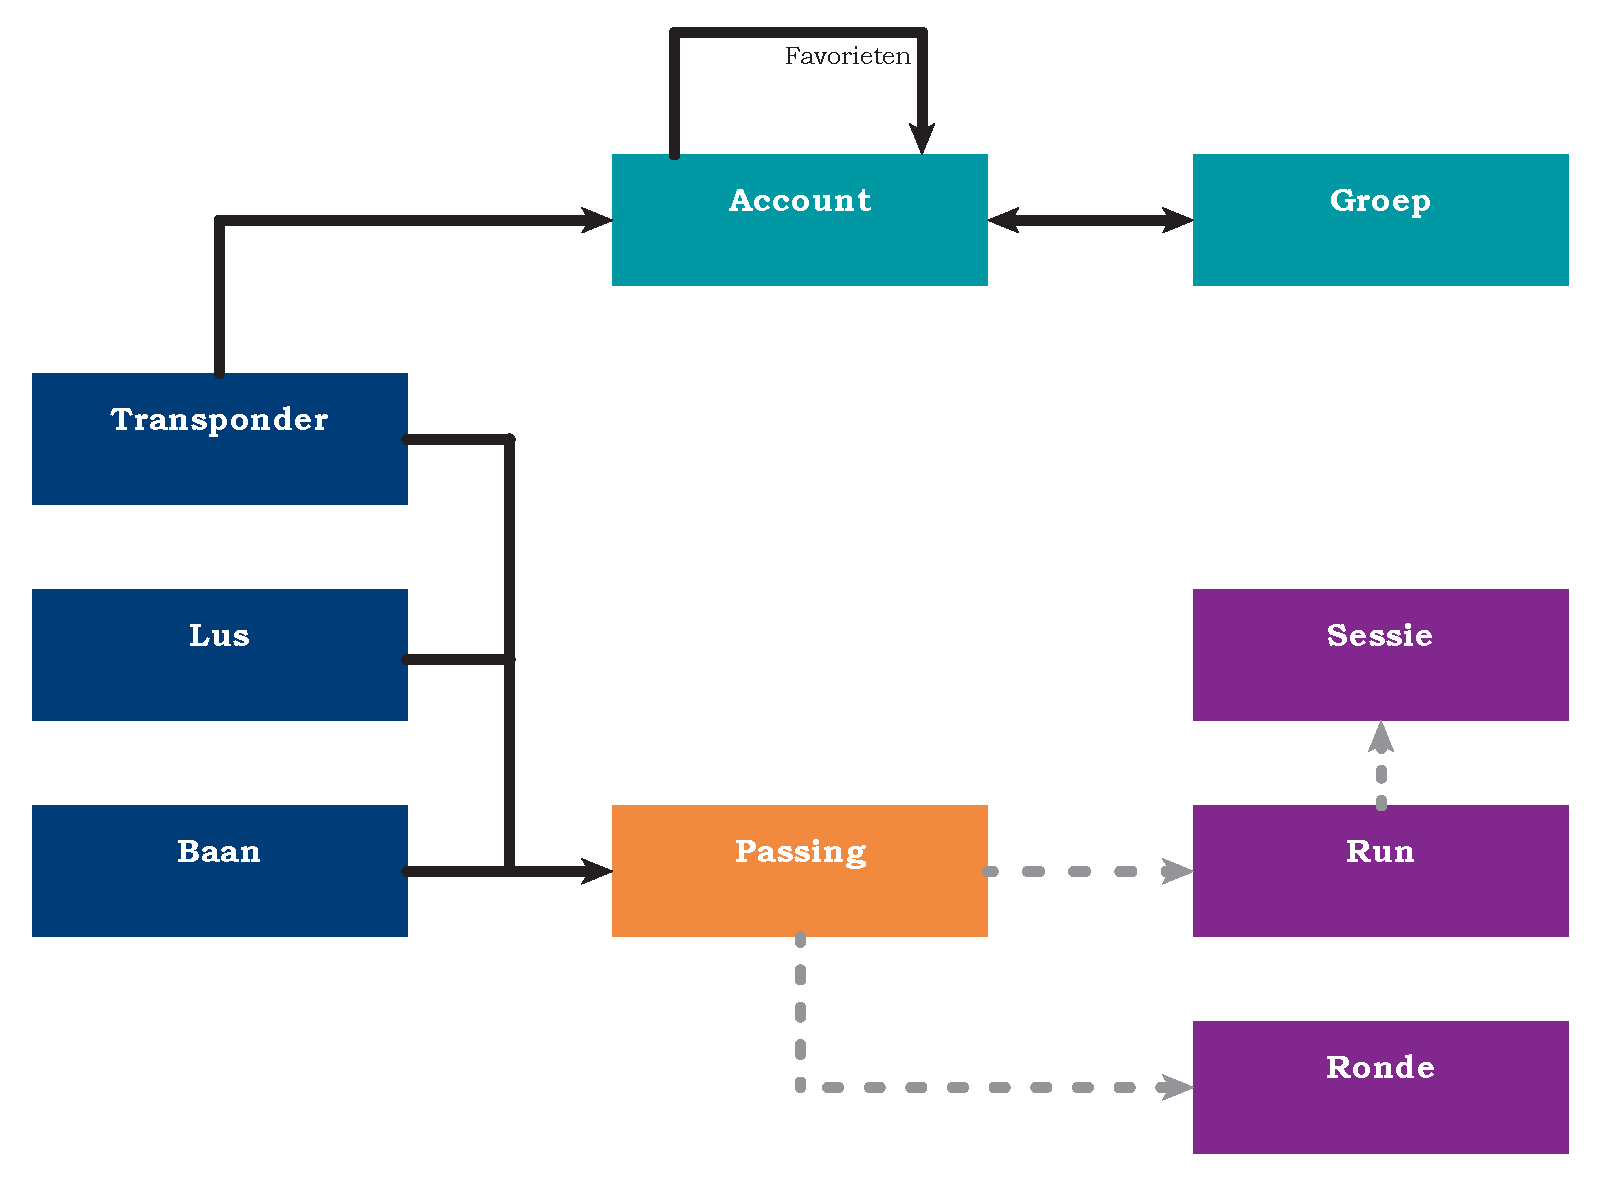
\includegraphics[width=0.8\textwidth]{style/images/Entiteiten}
\caption{Entiteiten binnen de applicatie}
\label{fig:entities}
\end{figure}


Wanneer een Passing ons systeem binnenkomt proberen we deze te koppelen aan een gebruiker. Als Passing bij een voor ons onbekende transponder hoort slaan we de Passing op en verwerken we hem later, als we de betreffende transponder wel kennen. Dit kan gebeuren als een gebruiker met terugwerkende kracht een transponder koppelt aan zijn account. Elke gebruikersaccount heeft dus een lijst met transponders en vanaf wanneer tot wanneer deze transponder in het bezit van de gebruiker was. Een transponder kan namelijk ook worden uitgeleend. Per tijdseenheid kan er per gebruiker maar één transponder zijn.

Aan de hand van een lijst met Passings kunnen we enkele berekeningen doen. Met deze berekeningen kunnen we bijvoorbeeld bepalen wanneer een training begint en eindigt. Een groep van de Passings van een training heet een Session. Binnen een training zijn weer Runs te onderscheiden. Runs zijn groepjes van passings waartussen een sporter niet uitreed. Een training in het baansporten kan er bijvoorbeeld bestaan uit het 5 keer rijden van 4 ronden, met tussendoor 2 ronden rust. Er zijn in dat geval binnen de sessie 4 runs te onderscheiden. In figuur~\ref{fig:sessions} is een training van Herman te zien. Bij Herman zijn rondetijden langzamer dan 40 seconden  geen actieve onderdelen, maar zijn uitrijd-rondjes. Dit is per sporter en sport verschillend, dus moet deze grens dynamisch bepaald worden of instelbaar zijn. In de figuur zijn de runs groen gekleurd.

\begin{figure}
\centering
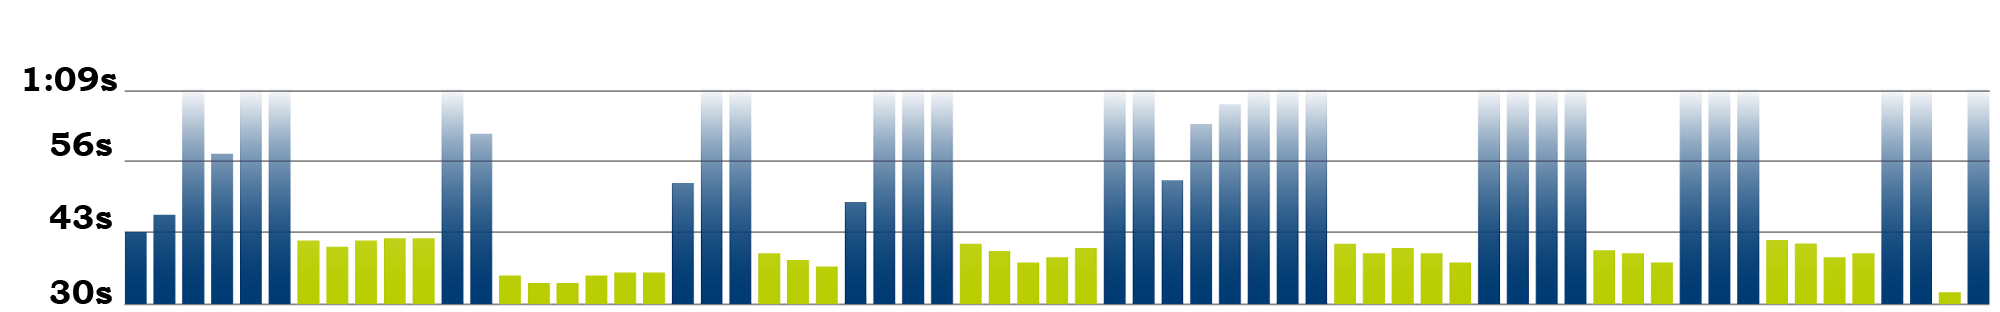
\includegraphics[width=1\textwidth]{style/images/MyLapsHerman}
\caption{De rondetijden tijdens een typische training; specifiek: training van Herman van 3 maart 2014}
\label{fig:sessions}
\end{figure}

\section{Database}
Zoals in figuur~\ref{fig:entities}, is een deel van onze data relationeel.. De gebruikers zijn gekoppeld aan transponders en transponders zijn gekoppeld aan Passings. Gebruikers kunnen deel uitmaken van groepen en kunnen een lijst met favoriete gebruikers hebben, welke ze willen volgen. Een deel van de data zullen we opslaan in een relationele database. Data die relatief weinig wordt aangepast zoals de gebruiker-accounts en bijbehorende transponders leent zich hier uitstekend voor. Met een \textit{join} is eenvoudig een lijst van transponders van een gebruiker op te halen. In figuur~\ref{fig:dbengines} is (een abstractie en deel van) de relationele data weergegeven in het blauw. De user-id's uit de account-tabel komen terug in de transponder-tabel.

\begin{figure}
\centering
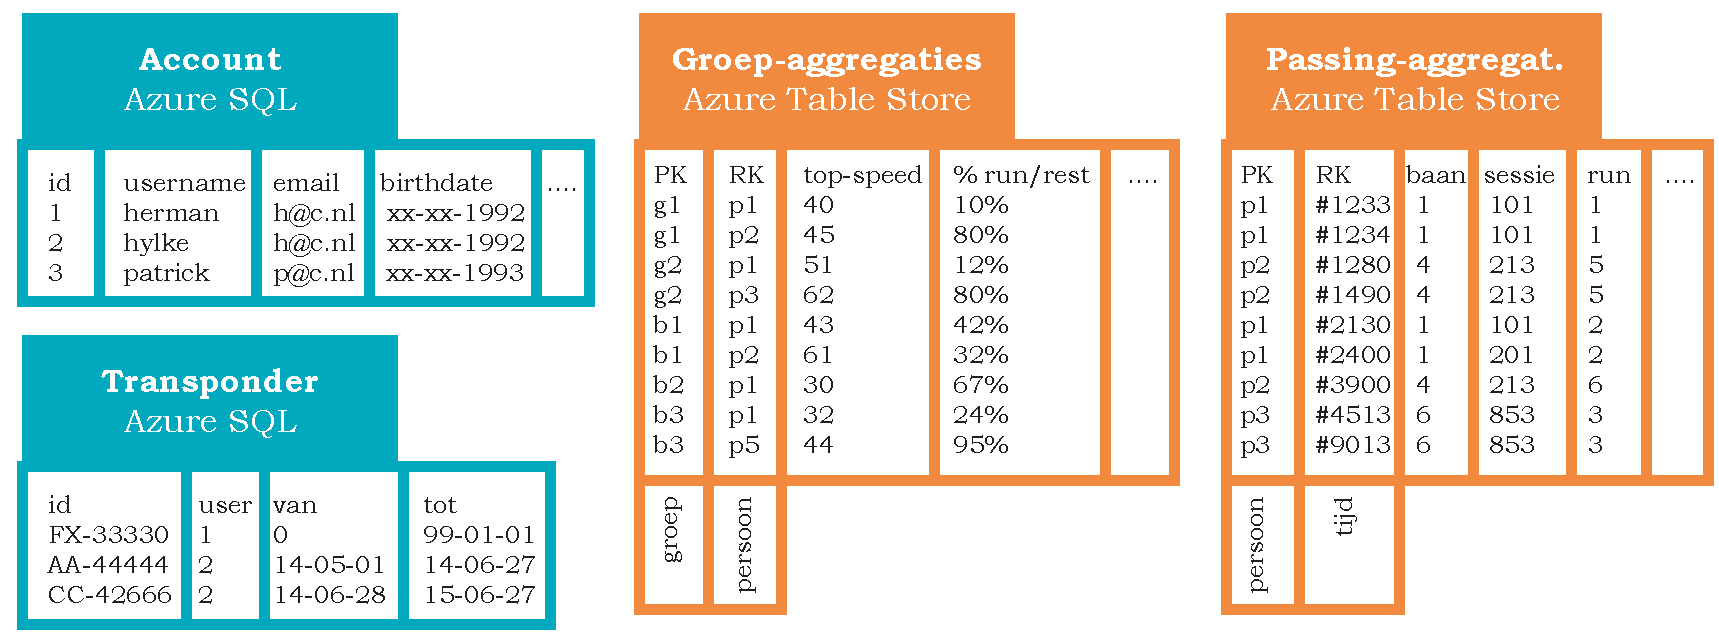
\includegraphics[width=\textwidth]{style/images/DBEngines}
\caption{Verschillende data, verschillende database engines}
\label{fig:dbengines}
\end{figure}

Naast de relationele data, genereren we met aggregaties heel veel nieuwe data, zoals de snelste rondetijd, de langste run, of de hoogste snelheid per persoon. Deze data is gebonden aan de groepen waarin een gebruiker zit en de banen waarop de Passing plaatsvond. In de meeting van 1 mei (Appendix~\ref{sec:meeting-1-mei}) is besproken om hiervoor de Azure Table Storage te gebruiken. Table Storage heeft twee keys per rij, de PartitionKey en de RowKey~\cite{azuretablestorage}. Wij slaan de (virtuele) groep op in de PartitionKey (PK) en de gebruikers in de RowKey (RK). Op die manier is snel voor een groep alle data op te halen, voor bijvoorbeeld een Leaderboard. Ook kan bij het opslaan van de aggregaties snel op de RowKey gefilterd worden. De verschillende aggregaties worden opgeslagen in verschillende kolommen. Azure Table Storage biedt de namelijk mogelijkheid arbitraire objecten te koppelen aan een PartitionKey en RowKey (de combinatie van de twee keys is uniek). In figuur~\ref{fig:dbengines} is (abstractie van) de platte data weergegeven in het oranje. In de Passing aggregatie tabel is de unieke key gebaseerd op de transponder en de timestamp van de Passing. Een transponder kan niet twee keer gedetecteerd worden op hetzelfde moment zonder dat het dezelfde Passing is. Aggregaties per passing zoals bij welke run en sessie de Passing hoorde slaan we hier in op.

Deze data wordt real-time verwerkt en doorgestuurd naar de client wanneer nodig. Om deze aggregaties snel en onafhankelijk van elkaar te laten verlopen, moet rekening worden gehouden met de mogelijkheid om bij pieken meerdere instanties van deze aggregatie-pijpen te draaien. Elke instantie ontvangt dan andere Passings. Om te zorgen dat de client altijd de laatste versie ontvangt wordt elke aggregatie vergezeld van de \textit{timestamp} van de laatste Passing. Als een client een aggregatie ontvangt met een oudere timestamp dan degene die hij al ontvangen heeft dan kan hij deze negeren.

\section{Architectuur}
In overleg met de opdrachtgever is gekozen voor een multi-layered architectuur met
vier lagen: de data-laag, business-laag, service-laag en de presentatie-laag. Deze 
architectuur garandeert een scheiding tussen verschillende stukken logica, zodat 
alle logica in de verantwoordelijke laag wordt uitgevoerd. In Figuur~\ref{fig:architecture} zijn alle layers en hun componenten weergegeven.

\begin{figure}
\centering
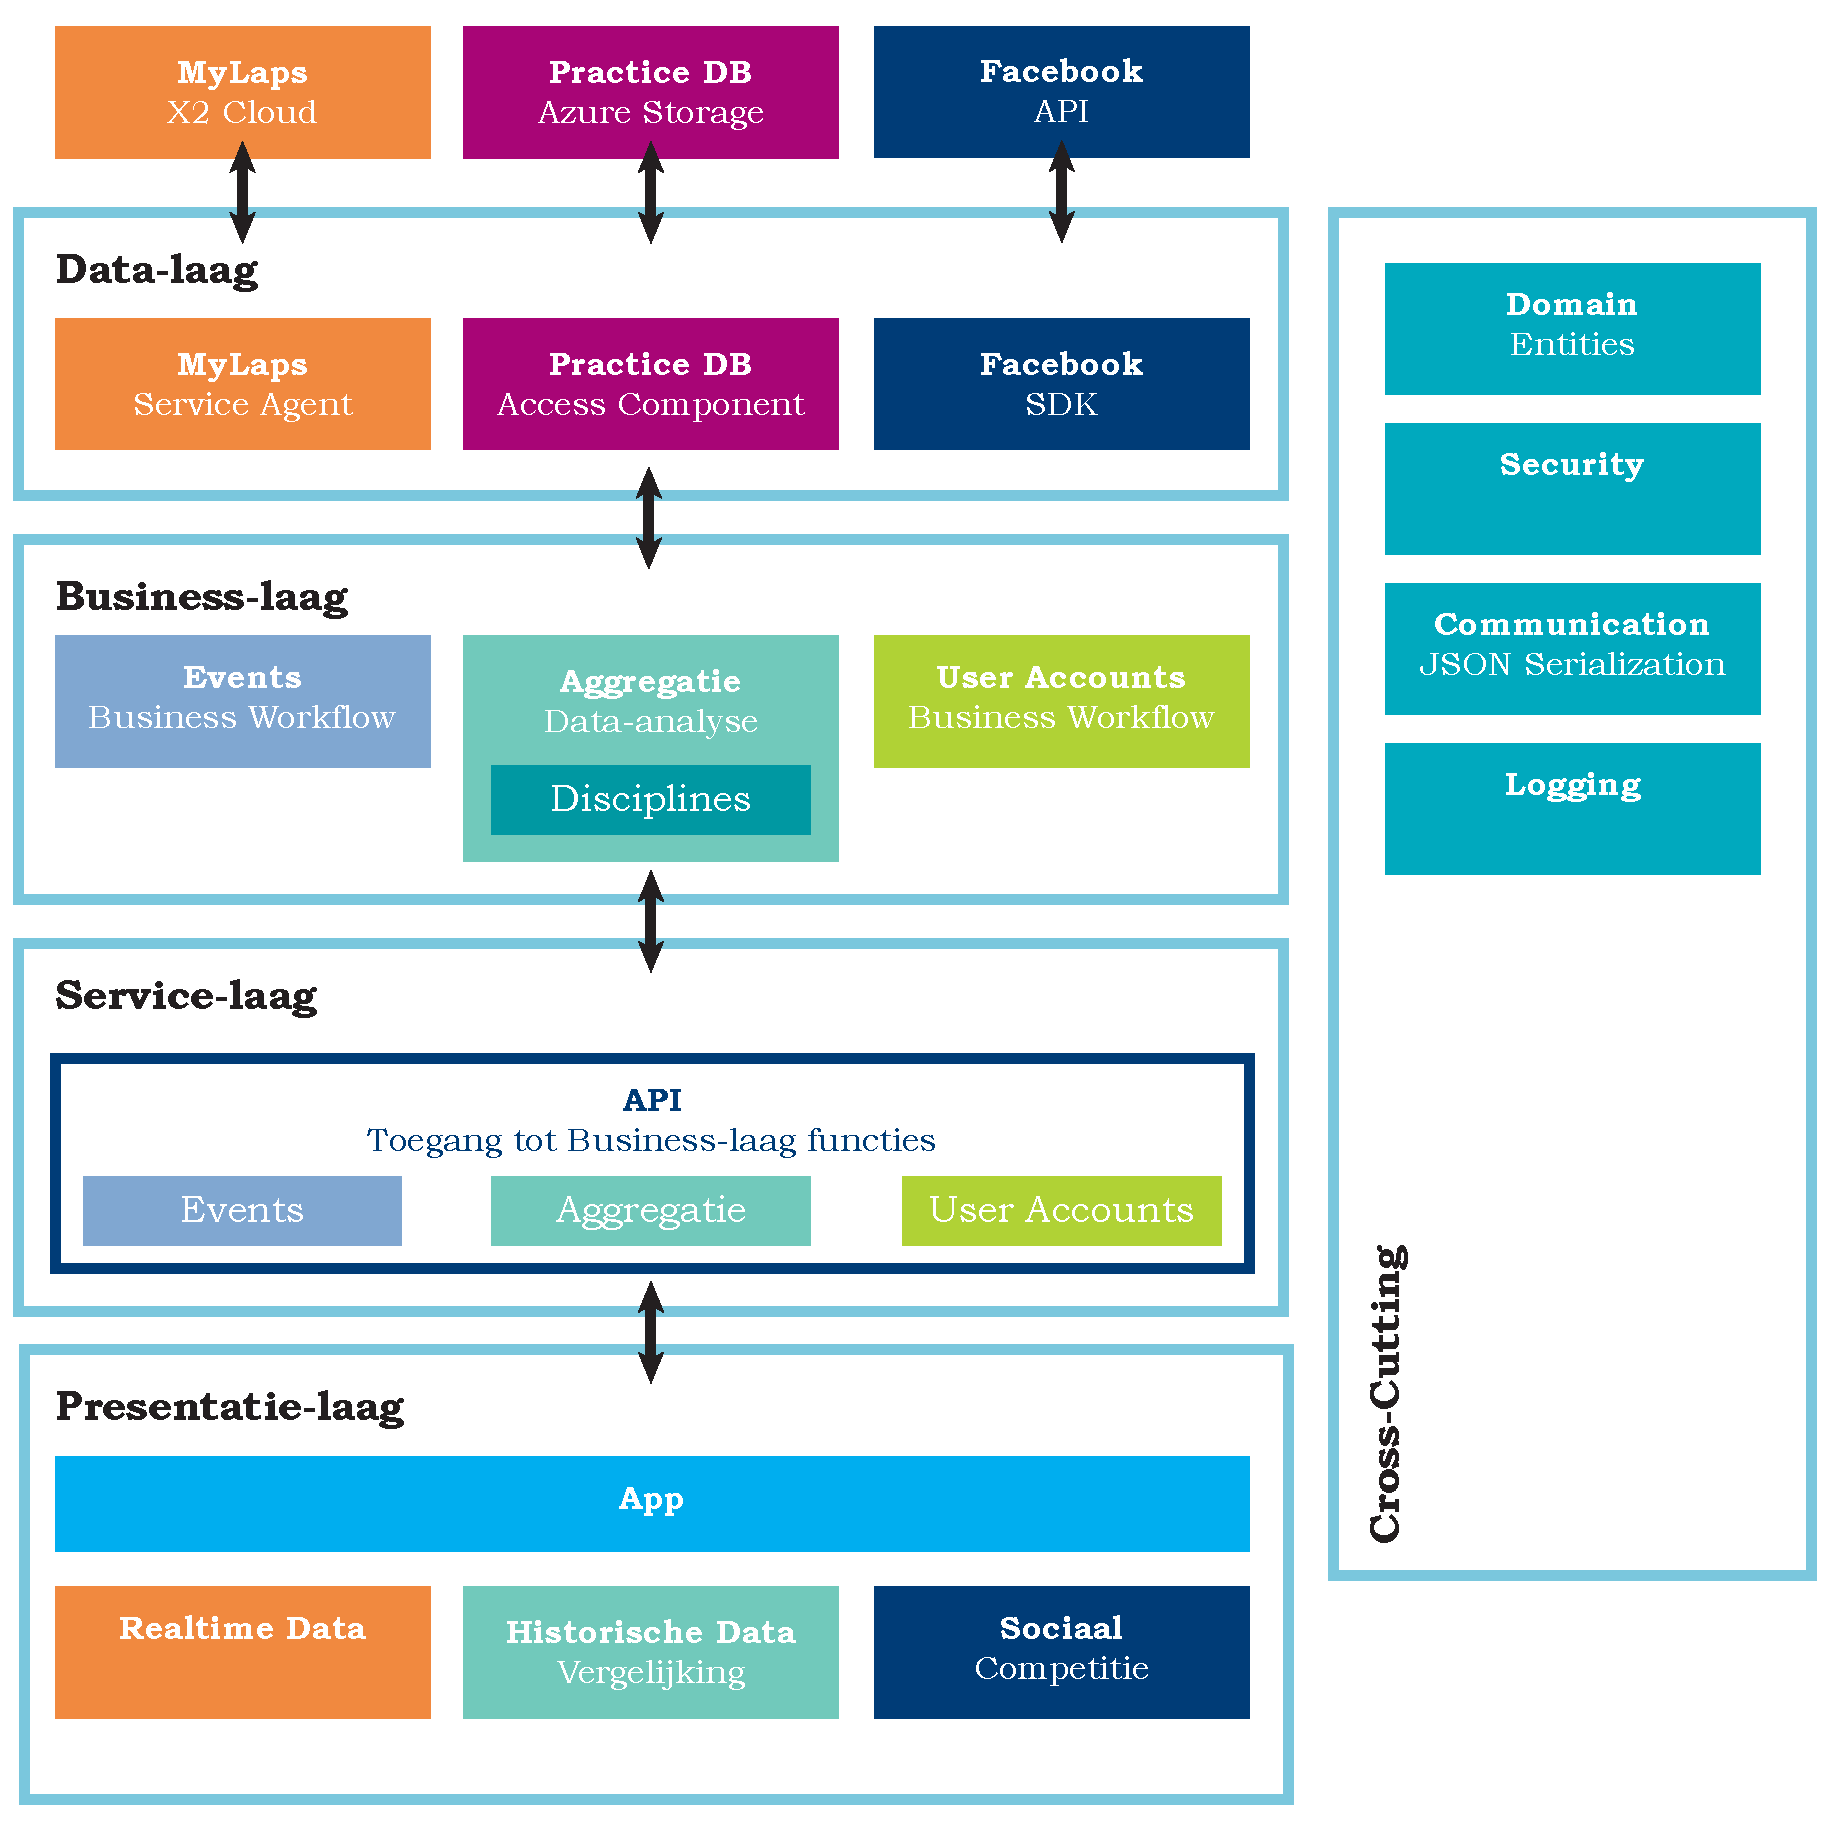
\includegraphics[width=\textwidth]{style/images/Architectuur}
\caption{Systeem architectuur}
\label{fig:architecture}
\end{figure}

De data-laag bevat componenten die een  verbinding kunnen maken met de databases en 
andere services zoals MyLaps Cloud en de Facebook API. De data-laag zet ruwe data 
uit de database om in domein entiteiten en levert deze af bij de business-laag.

De business-laag bevat alle workflows die op de server uitgevoerd moeten worden. 
De workflows zijn in drie categorieen op te delen. Als eerste de Aggregatie
componenten die diverse aggregaties kunnen uitvoeren op data uit de Practice
Database. Ten tweede is er de Event Workflow die bepaald wat er moet gebeuren als
er een event binnenkomt zoals bijvoorbeeld een doorkomst vanaf MyLaps. In het
geval van een doorkomst moet deze bijvoorbeeld worden opgeslagen in de Practice
Database en moeten de aggregaties een iteratie doorlopen. Als derde is er het User
Account component dat acties voor gebruikersacccounts mogelijk maakt. Zo is dit
component belast met het opslaan van nieuwe users, het inloggen met wachtwoord of
met Facebook, het beheren van groepen en het ophalen van vriendenlijsten.

De service-laag bevat de API. De diverse aanroepen die de clients nodig hebben
worden in de service-laag gekoppeld aan de goede workflow uit de business-laag. De
service-laag zorgt ook voor Caching, waar nodig.

De presentatie-laag bevindt zich in de mobiele applicaties. Deze toont de informatie uit de
service-laag. De presentatie-laag bevat bijvoorbeeld User Interface componenten, 
weergaves voor diverse data types en menu's. Naast de weergave zit er in de apps 
ook een stuk service-laag om te kunnen communiceren met de service-laag op de 
server.